
\section{Simulations}\label{sec-sim}


To assess the finite sample performance of the methods from Sections \ref{sec-test-shape} and \ref{sec-test-equality}, we conduct a number of simulations. We first investigate the test procedure from Section \ref{sec-test-shape}. The simulation design is set up to mimic the situation in the application example of Section \ref{subsec-data-1}: We generate data from the model $Y_t = m(t/T) + \varepsilon_t$ for different time series lengths $T$. The errors $\varepsilon_t$ are drawn from the AR(1) process $\varepsilon_t = a \varepsilon_{t-1} + \eta_t$, where $\eta_t$ are independent and normally distributed with mean $0$ and variance $\sigma_\eta^2$. We set $a = 0.267$ and $\sigma_\eta^2 = 0.35$, thus matching the estimated values obtained in the application of Section \ref{subsec-data-1}. To simulate data under the null $H_0: m^\prime = 0$, we let $m$ be a constant function. In particular, we set $m = 0$ without loss of generality. To generate data under the alternative, we consider the trend functions $m(u) = \beta \, (u - 0.6) \, 1(0.6 \le u \le 1)$ with $\beta = 1.25, 1.875, 2.5$. These functions are broken lines with a kink at $u = 0.6$ and different slopes $\beta$. The slope parameter $\beta$ corresponds to a trend with the value $m(1) = 0.4 \, \beta$ at the right endpoint $u = 1$. We thus consider broken lines with the values $m(1) = 0.5, 0.75, 1.0$. Inspecting the middle panel of Figure \ref{plot-results-app1}, these broken lines can be seen to resemble the local linear trend estimates in the real-data example of Section \ref{subsec-data-1} (where we neglect the nonlinearities of the local linear fits at the beginning of the observation period). 


To implement our test methods, we use the Epanechnikov kernel $K(x) = 0.75 \, (1 - x^2) \, 1(|x| \le 1)$ and define the set $\mathcal{G}_T$ of location-scale points $(u,h)$ to be 
\begin{equation}\label{grid-sim-app}
\mathcal{G}_T = \{(u, h): u = \frac{5k}{T} \text{ and } h = \frac{3+5l}{T} \text{ for some } k, l \in \mathbb{N}, k \le T/5, l \le T/20\}. 
\end{equation}
To estimate the long-run error variance $\sigma^2$, we employ the estimation procedure from Section \ref{subsec-error-var-ar}, setting the tuning parameters $L_1$ and $L_2$ to $18$ and $37$, respectively. The critical values are computed by simulating the $(1-\alpha)$ quantile $q_T^\prime(\alpha)$ of the statistic $\Phi^\prime_T$ defined in Section \ref{subsec-test-shape-test}. To do so, we simulate $1000$ values of the statistic $\Phi^\prime_T$ and compute their empirical $(1-\alpha)$ quantile. 


Tables \ref{tab:size_ll_shape} and \ref{tab:power_ll_shape} report the simulation results for the sample sizes $T=250,350,500, 1000$ and the confidence levels $\alpha = 0.01, 0.05, 0.10$. The sample size $T = 350$ is approximately equal to the time series length $359$ in the real-data example of Section \ref{subsec-data-1}. To produce our simulation results, we generate $S=10000$ samples for each time series length $T$ and carry out the multiscale test for each simulated sample. The entries of Tables \ref{tab:size_ll_shape} and \ref{tab:power_ll_shape} are computed as the number of simulations in which the test rejects divided by the total number of simulations. As can be seen from Table \ref{tab:size_ll_shape}, the actual size of the test is fairly close to the nominal target $\alpha$ even for small values of $T$, the accuracy increasing with the sample size. Hence, the test has approximately the correct size. Inspecting Table \ref{tab:power_ll_shape}, one can further see that the test has reasonable power properties. For the smallest value $\beta = 1.25$, the deviation from the null is quite small, making it hard for the test to detect the alternative. As a consequence, the power is only moderate in this case. When we move further away from the null by increasing the slope parameter $\beta$, the power of the test quickly increases. In addition, it can also be seen to quickly get larger as the sample size grows. 
 

\begin{table}[t]
\footnotesize{
\begin{center}
\caption{Size of the multiscale test from Section \ref{sec-test-shape} for different sample sizes $T$ and nominal sizes $\alpha$.}
\label{tab:size_ll_shape}
\renewcommand{\arraystretch}{1.2}
% latex table generated in R 3.4.3 by xtable 1.8-2 package
% 
\begin{tabular}{cccc}
  \hline
  & \multicolumn{3}{c}{nominal size $\alpha$} \\
 $T$ & 0.01 & 0.05 & 0.1 \\
 \hline
250 & 0.004 & 0.022 & 0.082 \\ 
  350 & 0.007 & 0.031 & 0.067 \\ 
  500 & 0.011 & 0.056 & 0.086 \\ 
  1000 & 0.011 & 0.060 & 0.098 \\ 
   \hline
\end{tabular}

\end{center}}
\end{table}

\begin{table}[t]
\footnotesize{
\begin{center}
\caption{Power of the multiscale test from Section \ref{sec-test-shape} for different sample sizes $T$ and nominal sizes $\alpha$. Each panel corresponds to a different slope parameter $\beta$.}\label{tab:power_ll_shape}
\begin{subtable}[b]{0.32\textwidth}
\centering
\caption{$\beta = 1.25$}\label{tab:power_050_ll_shape}
\renewcommand{\arraystretch}{1.2}
% latex table generated in R 3.4.3 by xtable 1.8-2 package
% 
\begin{tabular}{cccc}
  \hline
  & \multicolumn{3}{c}{nominal size $\alpha$} \\
 $T$ & 0.01 & 0.05 & 0.1 \\
 \hline
250 & 0.107 & 0.223 & 0.358 \\ 
  350 & 0.216 & 0.374 & 0.500 \\ 
  500 & 0.280 & 0.554 & 0.678 \\ 
  1000 & 0.756 & 0.910 & 0.935 \\ 
   \hline
\end{tabular}

\end{subtable}
\begin{subtable}[b]{0.32\textwidth}
\centering
\caption{$\beta = 1.875$}\label{tab:power_075_ll_shape}
\renewcommand{\arraystretch}{1.2}
% latex table generated in R 3.4.3 by xtable 1.8-2 package
% 
\begin{tabular}{cccc}
  \hline
  & \multicolumn{3}{c}{nominal size $\alpha$} \\
 $T$ & 0.01 & 0.05 & 0.1 \\
 \hline
250 & 0.365 & 0.582 & 0.709 \\ 
  350 & 0.644 & 0.779 & 0.845 \\ 
  500 & 0.784 & 0.942 & 0.976 \\ 
  1000 & 0.997 & 1.000 & 1.000 \\ 
   \hline
\end{tabular}

\end{subtable}
\begin{subtable}[b]{0.32\textwidth}
\centering
\caption{$\beta = 2.5$}\label{tab:power_100_ll_shape}
\renewcommand{\arraystretch}{1.2}
% latex table generated in R 3.4.3 by xtable 1.8-2 package
% 
\begin{tabular}{cccc}
  \hline
  & \multicolumn{3}{c}{nominal size $\alpha$} \\
 $T$ & 0.01 & 0.05 & 0.1 \\
 \hline
250 & 0.717 & 0.875 & 0.928 \\ 
  350 & 0.933 & 0.977 & 0.989 \\ 
  500 & 0.989 & 0.999 & 1.000 \\ 
  1000 & 1.000 & 1.000 & 1.000 \\ 
   \hline
\end{tabular}

\end{subtable}
\end{center}}
\end{table}


We next turn to the test methods from Section \ref{sec-test-equality}. The simulation design extends the setup from above. We generate data from the model $Y_{it} = m_i(t/T) + \varepsilon_{it}$, where the number of time series is set to $n = 30$ and we consider different time series lengths $T$. For each $i$, the errors $\varepsilon_{it}$ are drawn from the AR(1) model $\varepsilon_{it} = a \varepsilon_{i,t-1} + \eta_{it}$, where as before $a = 0.267$ and the innovations $\eta_{it}$ are i.i.d.\ normally distributed with mean $0$ and variance $0.35$. To generate data under the null $H_0: m_1 = \ldots = m_n$, we let $m_i = 0$ for all $i$ without loss of generality. To produce data under the alternative, we define $m_1(u) = \beta \, (u - 0.6) \, 1(0.6 \le u \le 1)$ with $\beta = 1.25, 1.875, 2.5$ and set $m_i = 0$ for all $i \ne 1$. Hence, all trend functions are the same except for $m_1$ which is a broken line as in the previous simulations. 


The test is implemented analogously as above. We in particular work with an Epanechnikov kernel and the grid $\mathcal{G}_T$ defined in \eqref{grid-sim-app}. Moreover, the long-run error variances $\sigma_i^2$ are estimated by the procedure from Section \ref{subsec-error-var-ar} with $L_1 = ??$ and $L_2 = ??$. The simulation results are reported in Tables ?? and ??. [\textcolor{red}{Discuss results!}]


We finally investigate the finite sample performance of the clustering algorithm from Section \ref{subsec-test-equality-clustering}. To do so, we partition the $n = 30$ time series into $N=3$ groups, each containing $10$ time series. Specifically, we set $G_1 = \{1,\ldots,10\}$, $G_2 = \{11,\ldots,20\}$ and $G_3 =  \{21,\ldots,30\}$. Moreover, we define the group-specific trend functions $g_1$, $g_2$ and $g_3$ by $g_1(u) = 0$, $g_2(u) =  2.5 \cdot (u - 0.6) \, 1(0.6 \le u \le 1)$ and $g_3(u) =  -2.5 \cdot (u - 0.6) \, 1(0.6 \le u \le 1)$. In order to compute our estimators of the groups $G_1$, $G_2$, $G_3$ and their number $N = 3$, we use the same implementation as before. The estimation results are reported in Tables ??. [\textcolor{red}{Discuss results!}]   



\section{Applications}\label{sec-data}


In what follows, we illustrate the multiscale methods from Sections \ref{sec-test-shape} and \ref{sec-test-equality} by two real-data examples. In the first example, we apply the test method from Section \ref{sec-test-shape} to a long time series of temperature data from Central England. In the second, we analyse a sample of temperature time series from 34 different weather stations in Great Britain with the help of the methods from Section \ref{sec-test-equality}. 


\begin{figure}[t]
\centering
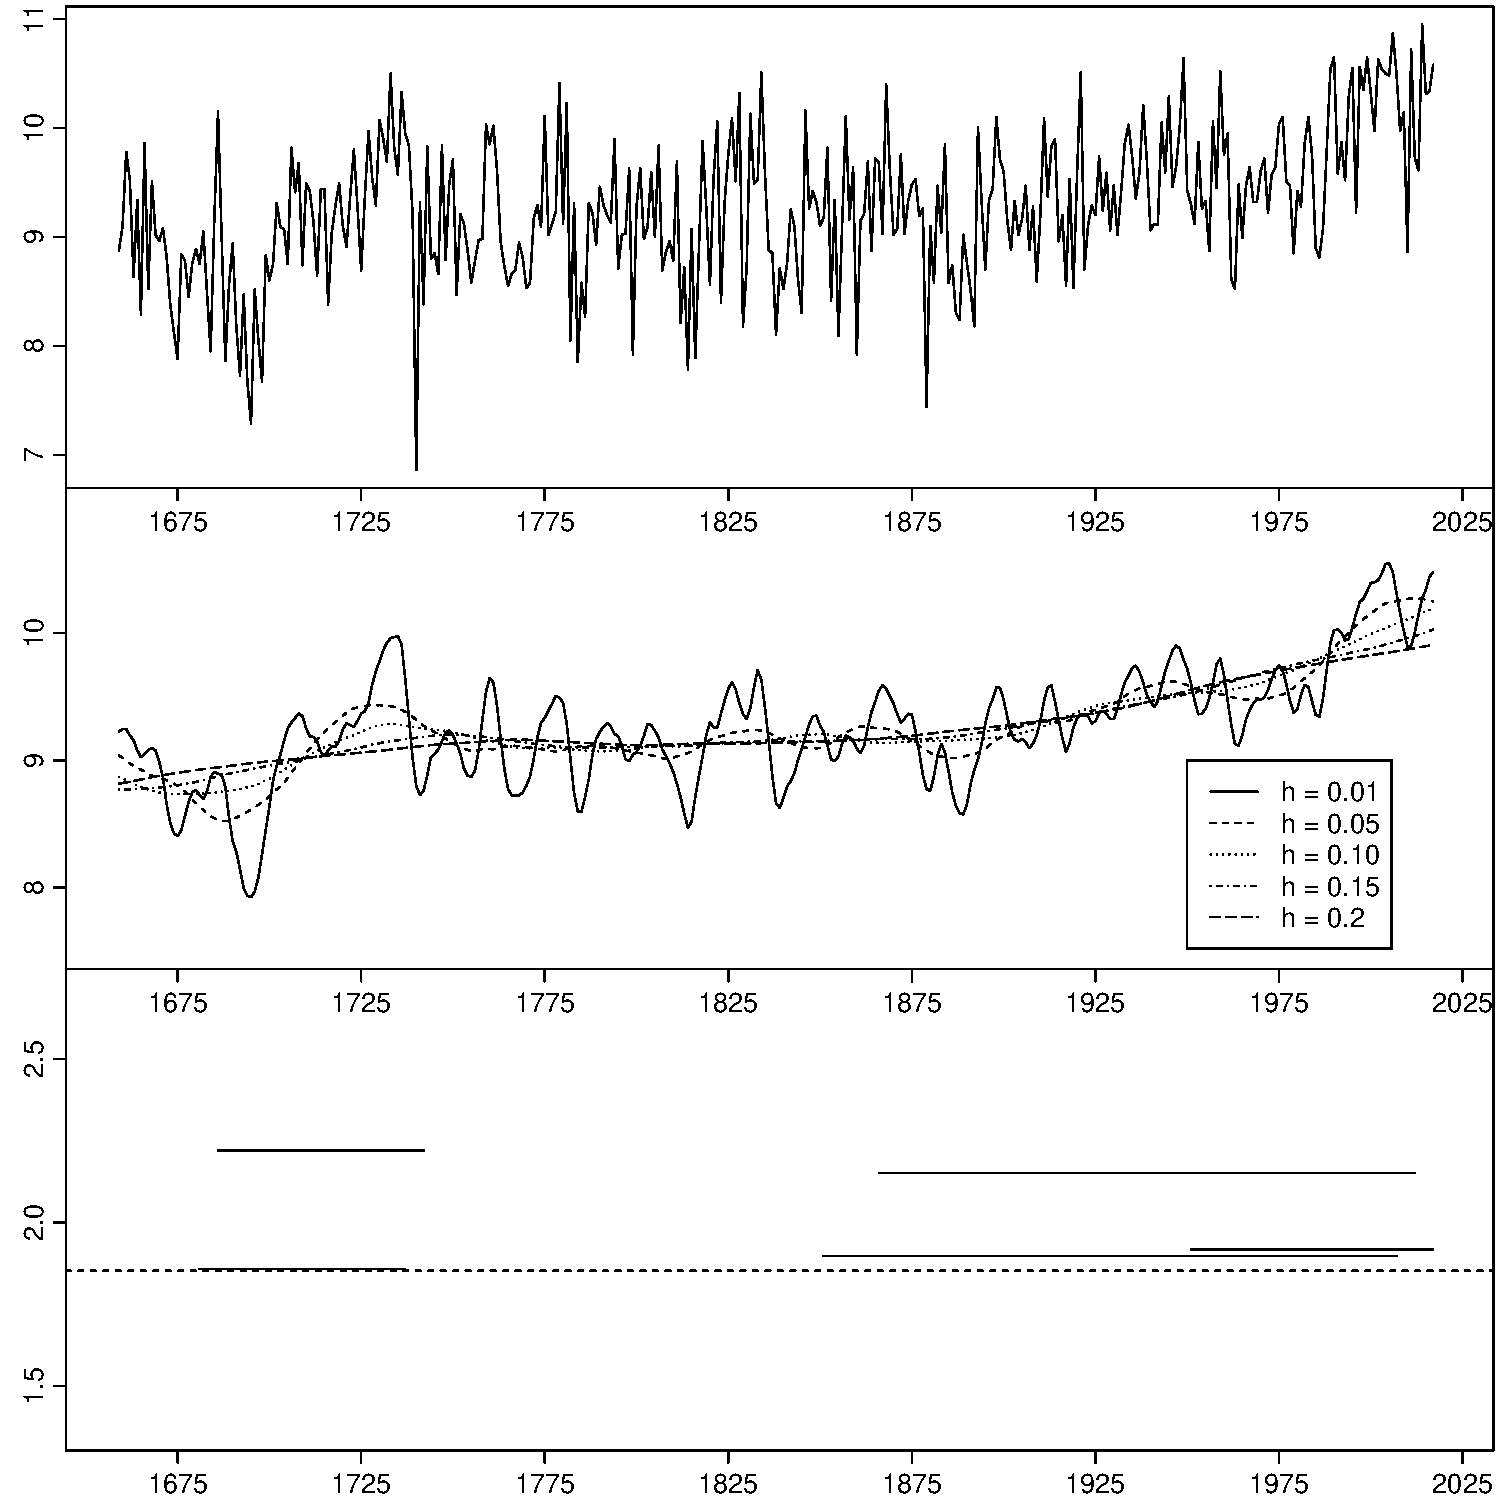
\includegraphics[width=0.8\textwidth]{Plots/threegraphics_testing_constant_method_ll.pdf}
\vspace{0.2cm}

\caption{Summary of the application results from Section \ref{subsec-data-1}. The upper panel shows the Central England mean temperature time series. The middle panel depicts local linear kernel estimates of the time trend for a number of different bandwidths $h$. The lower panel presents the minimal intervals in the set $\Pi_T^+$ produced by the multiscale test.}\label{plot-results-app1}
\end{figure}


\subsection{Analysis of Central England temperature data}\label{subsec-data-1} 


The analysis of time trends in long temperature records is an important task in climatology. Information on the shape of the trend is needed in order to better understand long-term climate variability. The Central England temperature record is the longest instrumental temperature time series in the world. It is a valuable asset for analysing climate variability over the last few hundred years. The data is publicly available on the webpage of the UK Met Office, a United Kingdom national weather service. A detailed description of the data can be found in \cite{Parker1992}. For our analysis, we use the dataset of yearly mean temperatures which consists of $T=359$ observations covering the years from $1659$ to $2017$. We assume that the data follow the nonparametric trend model 
\[ Y_t = m\Big(\frac{t}{T}\Big) + \varepsilon_t, \]
where $m$ is the unknown time trend of interest. The error process $\{ \varepsilon_t \}$ is supposed to have the AR(1) structure $\varepsilon_t = a \varepsilon_{t-1} + \eta_t$, where $\eta_t$ are i.i.d.\ innovations with mean $0$ and variance $\sigma_\eta^2$. As pointed out in \cite{Mudelsee2010}, this is a quite common error model for discrete climate time series. We estimate the unknown parameters $a$ and $\sigma_\eta^2$ by the procedure from Section \ref{subsec-error-var-ar} which yields estimates $\widehat{a} \approx 0.5$ and $\widehat{\sigma}_\eta^2 \approx 0.6$. As a robustness check, we have repeated the analysis with AR(2) and AR(3) errors. As the results are very similar, we have however not reported them here. Alternatively, one could of course select the AR order by an information criterion.   


We use our multiscale method from Section \ref{sec-test-shape} to test the null hypothesis $H_0: m^\prime = 0$, that is, the hypothesis that $m$ is constant. To do so, we set the significance level to $\alpha = 0.05$ and implement the test in exactly the same way as in the simulations of Section \ref{sec-sim}. The results are presented in Figure \ref{plot-results-app1}. The upper panel shows the raw temperature time series, whereas the middle panel depicts local linear kernel estimates of the trend $m$ for different bandwidths $h$. As one can see, the shape of the estimated time trend strongly differs with the chosen bandwidth. When the bandwidth is very small, there are many local increases and decreases in the estimated trend. When the bandwidth is very large, most of these local variations get smoothed out. Hence, by themselves, the nonparametric fits do not give much information on whether the trend $m$ is increasing or decreasing in certain time regions. 


Our multiscale test provides this kind of information, which is summarized in the lower panel of Figure \ref{plot-results-app1}. The plot depicts the minimal intervals contained in the set $\Pi_T^+$ which is defined in Section \ref{subsec-test-shape-theo}. The set of intervals $\Pi_T^-$ is empty in the present case. The height at which a minimal interval $I_{u,h} = [u-h,u+h] \in \Pi_t^+$ is plotted indicates the value of the corresponding (additively corrected) test statistic $\widehat{\psi}^\prime_T(u,h) - \lambda(h)$. The dashed line specifies the critical value $q_T^\prime(\alpha)$, where $\alpha = 0.05$ as already mentioned above. According to Proposition \ref{prop-test-shape-2}, we can make the following simultaneous confidence statement about the collection of minimal intervals in $\Pi_T^+$. We can claim, with confidence of about $95\%$, that the trend function $m$ has some increase on each minimal interval. In particular, we can claim with this confidence that there has been some upward movement in the trend both on the interval from ?? to ?? and on the interval from ?? to 2017. 
%As the minimal intervals cover the time period from ?? to 2017, we can in particular claim with simultaneous confidence of at least $95\%$, that there has been some upward movement in the trend both in the interval from ?? and ?? from ?? onwards. 
On the other hand, as the set $\Pi_T^-$ is empty, there is no evidence of some downward movement of the trend.  


To sum up, our multiscale test provides evidence that there have been some upward movements in the trend in the course of the observation period from $1659$ to $2017$. In particular, we can claim with confidence of around $95\%$, that there has been some increase in the trend within the time window from $1951$ to $2017$. 




\subsection{Analysis of UK weather station data}
